\chapter{\label{chap:spelunky}Spelunky}
Spelunky\footnote{http://www.spelunkyworld.com/original.html} é um jogo onde o
jogador incorpora um aventureiro que decide explorar uma caverna misteriosa. O
local contém tesouros, mas também está repleto de perigos. O objetivo principal
do jogador é explorar estas cavernas subterrâneas e coletar a maior quantia de
tesouros possível enquanto evita ser abatido pelos diversos inimigos e
armadilhas espalhadas pelo ambiente. A Figura \ref{fig:spelunky-gameplay}
ilustra uma partida do jogo.

\begin{figure}[htb!]
\centering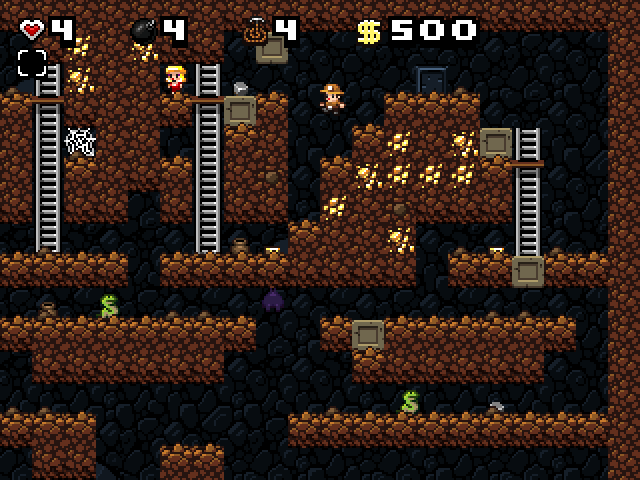
\includegraphics[width=.65\textwidth]{fig/spelunky-pc-screen.png}
\caption {\label{fig:spelunky-gameplay}Exemplo de partida de spelunky, mostrando
elementos do jogo como o jogador, a caverna, os inimigos, os tesouros, entre
outros.} \end{figure}

O jogo se enquadra no gênero \textit{platformer}, estilo de jogo que envolve
guiar um personagem através de plataformas suspensas e obstáculos para obter
progresso no jogo. Também faz uso de alguns dos elementos-chave do gênero
\textit{roguelike} -- tipo de jogos que se popularizou na década de 80
caracterizados por sua dificuldade, enfoque em exploração de ambientes e
narrativa fantasiosa --, como \textbf{geração procedural} e \textbf{morte
permanente}. Os níveis de Spelunky são gerados proceduralmente, ou seja, utiliza
um algoritmo capaz de gerar automáticamente os elementos que irão compor o
nível. Isto significa que não existe uma maneira de se memorizar estratégias
específicas de um mapa em Spelunky, pois ao início de cada partida o mapa é
gerado de maneira única e os tesouros, itens e obstáculos são dispostos de
maneira diferente, fazendo com que o jogador tenha que aprender a lidar com os
elementos do jogo de forma individual, combinar este conhecimento e estabelecer
uma estratégia para vencer seus obstáculos e ser bem sucedido. A seção
\ref{section:spelunky-procgen} explica em maiores detalhes o algoritmo utilizado
para geração procedural. Além disso, o jogo conta com o conceito de morte
permanente, que faz com que o jogador, ao ter seus pontos de vida esgotados,
tenha que recomeçar o jogo desde seu início, perdendo todo o progresso obtido
até então.

\section{\label{section:spelunky-goals}Objetivos}
% objetivo principal: derrotar Olmec e chegar ao fim do jogo
% objetivos secundários: tesouro, tempo, abates, salvamentos

\section{\label{section:spelunky-controls}Controle do Personagem}
% possiveis acoes que o jogador pode executar

\section{\label{section:spelunky-procgen}Algoritmo de Geração Procedural de
Níveis}
% entrar em detalhes

\section{\label{section:spelunky-obstacles}Obstáculos}
% inimigos (listar)
% armadilhas (listar)
% ambiente (quedas, lava, etc.)

\section{\label{section:spelunky-items}Itens}
% três categorias diferentes: consumíveis, acessórios e armas
% listar todos e dar breve explicação

\section{\label{section:spelunky-dev}Desenvolvimento e Distribuição}
O jogo foi desenvolvido por Derek Yu -- utilizando o motor de desenvolvimento de
jogos \textit{GameMaker} (Versão 8.0 Pro) -- e lançado gratuitamente para a
plataforma \textit{Windows} em dezembro de
2008\footnote{https://forums.tigsource.com/index.php?topic=4017}. No fim de
2009, o criador optou por liberar o código fonte do jogo, permitindo sua
distribuição não-comercial e
modificação\footnote{http://www.spelunkyworld.com/files/COPYING.txt}. A
liberação do código fonte de Spelunky pode ser considerada um marco muito
importante, pois permitiu que fossem criadas modificações para o jogo. Estas
modificações, que podem ser encontradas no fórum oficial da
\textit{Mossmouth}\footnote{http://mossmouth.com/forums/index.php} -- empresa
desenvolvedora de jogos criada por Derek Yu --, são correções de \textit{bugs},
mapas customizados ou até mesmo modos de jogo completamente diferentes do jogo
original. Pode-se dizer que dar esta liberdade para a comunidade do jogo é um
dos fatores que ajuda a manter sua base de jogadores e atraem novos jogadores
até hoje.

O motor GameMaker disponibiliza diversas ferramentas que facilitam o trabalho
do desenvolvedor. Contando com funcionalidades como editores de
\textit{scripts}\footnote{Código desenvolvido para o controle dos
comportamentos dos elementos do jogo.} e de \textit{sprites}\footnote{Elementos
visuais do jogo, tais como o personagem, o fundo, os inimigos. Representados
como uma ou mais imagens, permitindo que as mesmas sejam animadas.},
gerenciadores de eventos, entre
outras\footnote{http://sandbox.yoyogames.com/downloads/docs/gmaker80.pdf}, o
GameMaker oferece um ótimo suporte ao desenvolvedor para a criação de jogos. O
motor disponibiliza uma linguagem de programação própria para seus
\textit{scripts}, a \textit{GameMaker Language}, ou \textit{GML}.
